\documentclass[11pt,a4paper]{article}
\usepackage[hyperref]{emnlp2020}
\usepackage{times}
\usepackage{latexsym}
\renewcommand{\UrlFont}{\ttfamily\small}
\usepackage{cancel}
\usepackage{microtype}
\usepackage[algo2e]{algorithm2e} 
\aclfinalcopy \usepackage{algorithm}
\usepackage{algorithmic}


\newcommand\BibTeX{B\textsc{ib}\TeX}

\usepackage{amssymb}
\usepackage{amsthm}
\newtheorem{theorem}{Theorem}[section]
\newtheorem{corollary}{Corollary}[theorem]
\newtheorem{lemma}[theorem]{Lemma}

\usepackage{graphicx}
\usepackage{amsmath}
\usepackage{amssymb}
\usepackage{multirow}
\usepackage{makecell}
\usepackage{url}
\newcommand{\bc}[1]{\textbf{[BING: #1]}}
\usepackage{subcaption}
\usepackage{verbatim}
\usepackage{url}
\usepackage{array}
\usepackage{balance}
\usepackage{color}
\usepackage{soul}
\usepackage{hyperref}
\newcolumntype{L}[1]{>{\raggedright\let\newline\\\arraybackslash\hspace{0pt}}m{#1}}
\setul{2pt}{2pt}

\usepackage{pifont}
\newcommand{\xmark}{\ding{55}}

\renewcommand{\vec}[1]{\mathbf{#1}}

\DeclareMathOperator*{\argmax}{arg\,max}
\DeclareMathOperator*{\argmin}{arg\,min}
\DeclareMathOperator*{\softmax}{softmax}

\usepackage{changepage}
\usepackage{booktabs, tabularx}
\usepackage{arydshln}


\newcommand{\bing}[1]{\textcolor{blue}{\textbf{[BING: #1]}}}


\usepackage{pgfplots}
\usepackage{breakurl}
\usepackage{times}
\usepackage{latexsym}
\hypersetup{colorlinks}
\usepackage{booktabs}

\usepackage{url}
\newcounter{Lcount}
\newcommand{\squishenum}{
\begin{list}{\arabic{Lcount}. }
{ \usecounter{Lcount}
\setlength{\itemsep}{0pt}
\setlength{\parsep}{0pt}
\setlength{\topsep}{0pt}
\setlength{\partopsep}{0pt}
\setlength{\leftmargin}{2em}
\setlength{\labelwidth}{1.5em}
\setlength{\labelsep}{0.5em} } }

\newcommand{\RNum}[1]{\uppercase\expandafter{\romannumeral #1\relax}}
\newcommand{\squishletter}{
\begin{list}{\alph{Lcount}. }
{ \usecounter{Lcount}
\setlength{\itemsep}{0pt}
\setlength{\parsep}{0pt}
\setlength{\topsep}{0pt}
\setlength{\partopsep}{0pt}
\setlength{\leftmargin}{2em}
\setlength{\labelwidth}{1.5em}
\setlength{\labelsep}{0.5em} } }

\newcommand{\squishlist}{
\begin{list}{}
{ \usecounter{Lcount}
\setlength{\itemsep}{0pt}
\setlength{\parsep}{0pt}
\setlength{\topsep}{0pt}
\setlength{\partopsep}{0pt}
\setlength{\leftmargin}{2em}
\setlength{\labelwidth}{1.5em}
\setlength{\labelsep}{0.5em} } }




\newcommand{\udensdash}[1]{\tikz[baseline=(todotted.base)]{
        \node[inner sep=1pt,outer sep=0pt] (todotted) {#1};
        \draw[densely dashed,thick] (todotted.south west) -- (todotted.south east);
    }}

\newcommand{\squishend}{
\end{list} }

\usepackage[export]{adjustbox}
\usepackage{tikz}
\usepackage{pgf}
\usepackage{tikz-qtree}
\usepackage{xcolor}
\usepackage{multirow}
\usetikzlibrary{arrows,decorations.pathmorphing,backgrounds,positioning,fit,petri,shapes.misc, arrows.meta,shapes.geometric,decorations.markings,calc,shadows.blur,decorations.pathreplacing,quotes,matrix,shapes.symbols,patterns}
\definecolor{fontgray}{RGB}{44, 62, 80}
\definecolor{myred}{RGB}{235, 47, 6} \definecolor{summertime}{RGB}{245, 205, 121}
\definecolor{darkgrass}{RGB}{0, 148, 50}
\definecolor{myblue}{RGB}{0, 168, 255}
\definecolor{mygray}{RGB}{158, 158, 158}
\definecolor{puffin}{RGB}{250, 152, 58}
\definecolor{lowpurple}{RGB}{210, 180, 222}
\definecolor{lowblue}{RGB}{102,178,255}
\definecolor{lowred}{RGB}{245, 183, 177}

\newcommand{\pluseq}{\mathrel{+}=}

\newcommand*{\affaddr}[1]{#1} \newcommand*{\affmark}[1][*]{\textsuperscript{#1}}
\newcommand*{\email}[1]{\texttt{#1}}



\title{Position-Aware Tagging for Aspect Sentiment Triplet Extraction}

\author{Lu Xu\affmark[* 1, 2]\thanks{ Equal contribution.  Lu Xu is under the Joint PhD Program between Alibaba and Singapore University of Technology and Design. The work was done when Hao Li was a PhD student in Singapore University of Technology and Design.},
\thanks {Accepted as a long paper in EMNLP 2020 (Conference on Empirical Methods in Natural Language Processing).} 
Hao Li\affmark[* 1, 3], Wei Lu\affmark[1], Lidong Bing\affmark[2]\\
\affaddr{\affmark[1] StatNLP Research Group, Singapore University of Technology and Design}\\
\affaddr{\affmark[2] DAMO Academy, Alibaba Group}~~ \affaddr{\affmark[3]ByteDance}\\
\tt{xu\_lu@mymail.sutd.edu.sg, hao.li@bytedance.com}\\
\tt{ luwei@sutd.edu.sg, l.bing@alibaba-inc.com}\\
}
\renewcommand\footnotemark{}
\date{}



\pgfplotsset{
    /pgfplots/area legend/.style={
        legend image code/.code={\draw[#1] (0cm,-0.1cm) rectangle (0.1cm,0.15cm);
    }
    }
}

\begin{document}
\maketitle
\begin{abstract}
Aspect Sentiment Triplet Extraction (ASTE) is the task of extracting the triplets of target entities, their associated sentiment, and opinion spans explaining the reason for the sentiment.
Existing research efforts mostly solve this problem using pipeline approaches, which break the triplet extraction process into several stages. 
Our observation is that the three elements within a triplet are highly related to each other, and this motivates us to build a joint model to extract such triplets using a sequence tagging approach.
However, how to effectively design a tagging approach to extract the triplets that can capture the rich interactions among the elements is a challenging research question.
In this work, we propose the first end-to-end model with a novel {\em position-aware} tagging scheme that is capable of jointly extracting the triplets.
Our experimental results on several existing datasets show that jointly capturing elements in the triplet using our approach leads to improved performance over the existing approaches.
We also conducted extensive experiments to investigate the model effectiveness and robustness\footnote{We release our code at \url{https://github.com/xuuuluuu/Position-Aware-Tagging-for-ASTE}}.


\end{abstract}




\section{Introduction}
\label{sec:intro}

Designing effective algorithms that are capable of automatically performing sentiment analysis and opinion mining is a challenging and important task in the field of natural language processing~\cite{pang2008opinion,liu2010sentiment,ortigosa2014sentiment,smailovic2013predictive,li2010using}.
Recently, Aspect-based Sentiment Analysis ~\cite{pontiki-EtAl:2014:SemEval} or Targeted Sentiment Analysis~\cite{mitchell2013open} which focuses on extracting target phrases as well as the sentiment associated with each target, has been receiving much attention.
In this work, we focus on a relatively new task -- Aspect Sentiment Triplet Extraction (ASTE) proposed by~\citet{peng2019knowing}. 
Such a task is required to extract not only the targets and the sentiment mentioned above, but also the corresponding opinion spans expressing the sentiment for each target.
Such three elements: a target, its sentiment and the corresponding opinion span, form a triplet to be extracted.
Figure~\ref{fig:example} presents an example sentence containing two targets in solid boxes.
Each target is associated with a sentiment, where we use  to denote the positive polarity,  for neutral, and  for negative.
Two opinion spans in dashed boxes are connected to their targets by arcs.
Such opinion spans are important, since they largely explain the sentiment polarities for the corresponding targets~\cite{qiu-etal-2011-opinion,yang-cardie-2012-extracting}.

\begin{figure}[t!]
		\centering
\adjustbox{max width=1.0\linewidth}{
			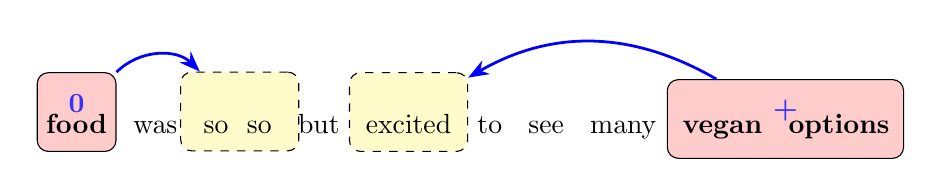
\begin{tikzpicture}[node distance=1.0mm and 1.0mm, >=Stealth, 
			wordnode/.style={draw=none, minimum height=5mm, inner sep=0pt},
			chainLine/.style={line width=1pt,->, color=blue},
			opinionbox/.style={draw=black, rounded corners, fill=yellow!20, dashed},
			targetbox/.style={draw=black, rounded corners, fill=red!20}
			]

			\matrix (sent1) [matrix of nodes, nodes in empty cells, execute at empty cell=\node{\strut};]
			{
				\textbf{food} & [1mm] was &[1mm] so & so & [1mm] but &  [1mm]  excited & [1mm] to & [1mm] see & [1mm] many & [1mm] \textbf{vegan} & [1mm] \textbf{options}\\
};
						
			\begin{pgfonlayer}{background}
			
			\node [targetbox, above=of sent1-1-1, yshift=-7mm, text height=-2mm, minimum height = 10mm, minimum width=10mm] (e1)  [] {\color{blue!80}\textbf{\textsc{0}}};	
			\node [opinionbox, above=of sent1-1-3, xshift=3mm, yshift=-6mm, text height=-5mm, minimum height = 10mm, minimum width=15mm] (o1)  [] {\color{blue!80}\textbf{\textsc{}}};
			
			\draw[chainLine,blue]   (e1) to[out=45,in=135] (o1);
			

			\node [targetbox, above=of sent1-1-10, xshift=8mm, yshift=-7mm, text height=-2mm, minimum height = 10mm, minimum width=30mm] (e2)  [] {\color{blue!80}\textbf{\textsc{+}}};			
			\node [opinionbox, above=of sent1-1-6, xshift=0mm, yshift=-7mm, text height=-5mm, minimum height = 10mm, minimum width=15mm] (o2)  [] {\color{blue!80}\textbf{\textsc{}}};
			
			\draw[chainLine,blue]   (e2) to[out=150,in=30] (o2);
				
			\end{pgfonlayer}
			
		
			
			\end{tikzpicture} 
		}
\caption{ASTE with targets in bold in solid squares, their associated sentiment on top, and opinion spans in dashed boxes. The arc indicates connection between a target and the corresponding opinion span.}
		\vspace{-2mm}
		\label{fig:example}
\end{figure}




\begin{figure*}[t!]
		\centering
\adjustbox{max width=1.0\linewidth}{
			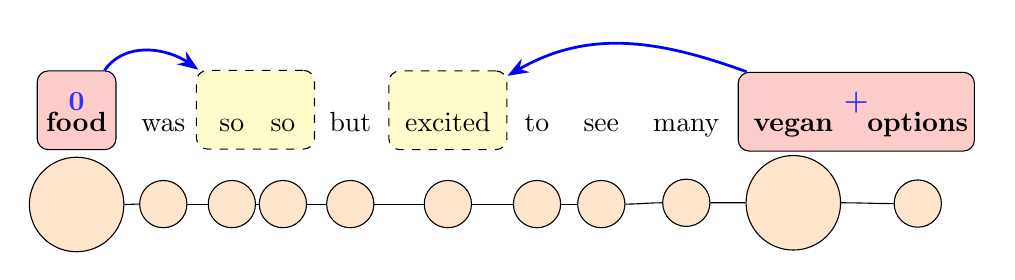
\begin{tikzpicture}[node distance=1.0mm and 1.0mm, >=Stealth, 
			wordnode/.style={draw=none, minimum height=5mm, inner sep=0pt},
			chainLine/.style={line width=1pt,->, color=blue},
			opinionbox/.style={draw=black, rounded corners, fill=yellow!20, dashed},
			targetbox/.style={draw=black, rounded corners, fill=red!20},
			BStag/.style={shape=circle, draw=black, rounded corners, fill=orange!20, minimum height=12mm, inner sep=0pt},
			MEOtag/.style={shape=circle, draw=black, rounded corners, fill=orange!20, minimum height=6mm, inner sep=0pt}
			]

\matrix (sent1) [matrix of nodes, nodes in empty cells, execute at empty cell=\node{\strut};]
			{
				\textbf{food} & [2mm] was &[2mm] so & [1mm]  so & [2mm] but &  [2mm]  excited & [2mm] to & [2mm] see & [2mm] many & [2mm] \textbf{vegan} & [2mm] \textbf{options}\\
};
			


\foreach \pos in {1}
				\node [BStag, below=of sent1-1-\pos, yshift=-0.9mm] (tag\pos)  [] {\color{black!80}\textsc{}};


\foreach \pos/\yoffset in {{2/-3.85},{3/-3.85},{4/-3.85},{5/-3.85},{6/-3.85},{7/-3.85},{8/-3.85},{9/-3}}
\node [MEOtag, below=of sent1-1-\pos, yshift=\yoffset mm] (tag\pos)  [] {\color{black!80}\textsc{}};
			
\node [BStag, below=of sent1-1-10, yshift=0mm] (tag10)  [] {\color{black!80}\textsc{}};
			
\node [MEOtag, below=of sent1-1-11, yshift=-3.1mm] (tag11)  [] {\color{black!80}\textsc{}};

			\foreach \pos/\npos in {{1/2},{2/3},{3/4},{4/5},{5/6},{6/7},{7/8},{8/9},{9/10},{10/11}}
				\draw[-]  (tag\pos) to[out=0,in=180] (tag\npos);
							
			
						
			\begin{pgfonlayer}{background}
			
			\node [targetbox, above=of sent1-1-1, yshift=-7mm, text height=-2mm, minimum height = 10mm, minimum width=10mm] (e1)  [] {\color{blue!80}\textbf{\textsc{0}}};	
			\node [opinionbox, above=of sent1-1-3, xshift=3mm, yshift=-6mm, text height=-5mm, minimum height = 10mm, minimum width=15mm] (o1)  [] {\color{blue!80}\textbf{\textsc{}}};
			
			\draw[chainLine,->]   (e1) to[out=55,in=145] (o1);
			

			\node [targetbox, above=of sent1-1-10, xshift=8mm, yshift=-6.3mm, text height=-2mm, minimum height = 10mm, minimum width=30mm] (e2)  [] {\color{blue!80}\textbf{\textsc{+}}};			
			\node [opinionbox, above=of sent1-1-6, xshift=0mm, yshift=-7mm, text height=-5mm, minimum height = 10mm, minimum width=15mm] (o2)  [] {\color{blue!80}\textbf{\textsc{}}};		
			
			\draw[chainLine,->]  (e2) to[out=160,in=30] (o2);
				
			\end{pgfonlayer}
			
			
			
			\end{tikzpicture} 
		}		\caption{The position-aware tagging scheme for the example instance.}
\label{fig:structure}
	\end{figure*}























This ASTE problem was basically untouched before, and the only existing work that we are aware of~\cite{peng2019knowing} employs a 2-stage pipeline approach.
At the first stage, they employ a unified tagging scheme which fuses the target tag based on the \footnote{ is a common tagging scheme for sequence labeling tasks, and  denotes ``begin, inside, outside, end and single'' respectively.} tagging scheme, and sentiment tag together.
Under such a unified tagging scheme, they proposed methods based on Long Short-Term Memory networks (LSTM) \cite{lstm97}, Conditional Random Fields (CRF) \cite{lafferty2001conditional} and Graph Convolutional Networks (GCN) \cite{kipf2017semi} to perform sequence labeling to extract targets with sentiment as well as opinion spans.
At the second stage, they use a classifier based on Multi-Layer Perceptron (MLP) to pair each target (containing a sentiment label) with the corresponding opinion span to obtain all the valid triplets. 


One important observation is that the three elements in a triplet are highly related to each other. 
Specifically, sentiment polarity is largely determined by an opinion span as well as the target and its context, and an opinion span also depends on the target phrase in terms of wording (e.g., an opinion span \textit{``fresh''} usually describes food targets instead of service).
Such an observation implies that jointly capturing the rich interaction among three elements in a triplet might be a more effective approach.
However, the  tagging scheme on which the existing approaches based comes with a severe limitation for this task:
such a tagging scheme without encoding any positional information fails to specify the connection between a target and its opinion span as well as the rich interactions among the three elements due to the limited expressiveness.
Specifically,   uses the tag  or  to represent the beginning of a target. For example, in the example sentence in Figure \ref{fig:example}, \textit{``vegan''} should be labeled with , but the tagging scheme does not contain any information to specify the position of its corresponding opinion \textit{``excited''}.
Using such a tagging scheme inevitably leads to an additional step to connect each target with an opinion span as the second stage in the pipeline approach.
{\color{black}The skip-chain sequence models~\cite{sutton2004collective, galley-2006-skip} are able to capture interactions between given input tokens which can be far away from each other.
However, they are not suitable for the ASTE task where the positions of targets and opinion spans are not explicitly provided but need to be learned.}




Motivated by the above observations, we present a novel approach that is capable of predicting the triplets jointly for ASTE. Specifically, we make the following contributions in this work:
\squishlist
\item  We present a novel position-aware tagging scheme that is capable of specifying the structural information for a triplet -- the connection among the three elements by enriching the label semantics with more expressiveness, to address the above limitation.
\item We propose a novel approach, \textbf{JET}, to \underline{J}ointly \underline{E}xtract the \underline{T}riplets based on our novel position-aware tagging scheme. 
Such an approach is capable of better capturing interactions among elements in a triplet by computing factorized features for the structural information in the ASTE task.
\item Through extensive experiments, the results show that our joint approach \textbf{JET} outperforms baselines significantly.
\squishend












    





\section{Our Approach}
Our objective is to design a model \textbf{JET} to extract the triplet of Target, Target Sentiment, and Opinion Span jointly.
We first introduce the new position-aware tagging scheme, followed by the model architecture. We next present our simple LSTM-based neural architecture for learning feature representations, followed by our method to calculate factorized feature scores based on such feature representations for better capturing the interactions among elements in a triplet.
Finally, we also discuss a variant of our model.






\subsection{Position-Aware Tagging Scheme}


To address the limitations mentioned above, we propose our position-aware tagging scheme by enriching expressiveness to incorporate position information for a target and the corresponding opinion span.
Specifically, we extend the tag  and tag  in the  tagging scheme to new tags respectively:\setlength{\abovedisplayskip}{0pt} \setlength{\abovedisplayshortskip}{0pt}
\setlength{\belowdisplayskip}{4pt} \setlength{\belowdisplayshortskip}{4pt}

where  with the sub-tag\footnote{We define the sub-tags of  as  and  respectively, and the sub-tags of  as themselves.}  still denotes the beginning of a target, and  with the sub-tag  denotes a single-word target.
Note that  denotes the sentiment polarity for the target, and   indicate the position information which are  the distances 
between the two ends of an opinion span and the starting position of a target respectively.
Here, we use the term ``{\em offset}'' to denote such  position information for convenience.
We keep the other tags , ,  as is.
In a word, we use sub-tags  for encoding targets,  for sentiment, and offsets for opinion spans under the new position-aware tagging scheme for the structural information.


For the example in Figure~\ref{fig:example}, under the proposed tagging  scheme, the tagging result is given in Figure~\ref{fig:structure}.
The single-word target \textit{``food''} is tagged with , implying the sentiment polarity for this target is neutral (0). 
Furthermore, the positive offsets  indicate that its opinion span is on the right and has distances of 2 and 3 measured at the left and right ends respectively, (i.e., \textit{``so so''}).
The second target is \textit{``vegan options''} with its first word tagged with  and the last word tagged with , implying the sentiment polarity is positive ().
Furthermore, the negative offsets  indicate that the opinion span \textit{``excited''} appears on the left of the target, and has distances of 4 and 4 measured at the left and right ends respectively, (i.e., \textit{``vegan''}).

\textcolor{black}{
Our proposed position-aware tagging scheme has the following theoretical property:
\begin{theorem} There is a one-to-one correspondence between a tag sequence and a combination of aspect sentiment triplets within the sentence as long as the targets do not overlap with one another, and each has one corresponding opinion span.\footnote{See the Appendix for detailed statistics on how often this condition is satisfied.}
\end{theorem} 
\begin{proof}
For a given triplet, we can use the following process to construct the tag sequence.
    First note that the sub-tags of our proposed tags , are . The standard  tagset is capable of extracting all possible targets when they do not overlap with one another. 
    Next, for each specified target, the position information  that specifies the position of its corresponding opinion span can be attached to the  (or ) tag, resulting in  (or ). Note that the opinion span can be any span within the sentence when  are not constrained. Finally, we assign each extracted target its sentiment polarity  by attaching it to the tag  (or ), resulting in  (or ). This construction process is unique for each combination of triplets. Similarly, given a tag sequence, we can reverse the above process to recover the combination of triplets.
\end{proof}
We would like to highlight that our proposed position-aware tagging scheme is capable of handling some special cases where the previous approach is unable to. For example, in the sentence \textit{``The salad is cheap with fresh salmon"}, there are two triplets, (\textit{``salad"}, \textit{``cheap with fresh salmon"}, positive)\footnote{We use the format (target, opinion spans, sentiment).} and (\textit{``salmon"}, \textit{``fresh"}, positive). The previous approach such as \cite{peng2019knowing}, which was based on a different tagging scheme, will not be able to handle such a case where the two opinion spans overlap with one another.}























			






			
						













			
			



\subsection{Our JET Model}



We design our novel \textbf{JET} model with CRF~\cite{lafferty2001conditional} and Semi-Markov CRF~\cite{sarawagi2004semi} based on our position-aware tagging scheme.
Such a model is capable of encoding and factorizing both token-level features for targets and segment-level features for opinion spans.


Given a sentence  with length , we aim to produce the desired output sequence  based on the  position-aware  tagging scheme.
The probability of  is defined as:
\setlength{\abovedisplayskip}{4pt} \setlength{\abovedisplayshortskip}{4pt}
\setlength{\belowdisplayskip}{4pt} \setlength{\belowdisplayshortskip}{4pt}

where  is a score function defined over the sentence  and the output structure , and  represents all the possible sequences under our position-aware tagging scheme with the offset constraint , indicating the maximum absolute value of an offset.
The score  is defined as:
\setlength{\abovedisplayskip}{4pt} \setlength{\abovedisplayshortskip}{4pt}
\setlength{\belowdisplayskip}{4pt} \setlength{\belowdisplayshortskip}{4pt}

where  returns the sub-tag of ,  represents the transition score: the weight of a ``transition feature'' -- a feature defined over two adjacent sub-tags  and , and  represents the factorized feature score with tag  at position .
In our model, the calculation of transition score  is similar to the one in CRF\footnote{We calculate the transition parameters among five sub-tags  for targets.}.
{\color{black}For the factorized feature score , we will explain computation details based on a simple LSTM-based neural network in the following two subsections. }
Such a factorized feature score is able to encode both token-level features as in standard CRF, segment-level features as in Semi-Markov CRF as well as the interaction among a target, its sentiment and an opinion span in a triplet.

\begin{figure}[t!]
		\centering
\adjustbox{max width=1.0\linewidth}{
			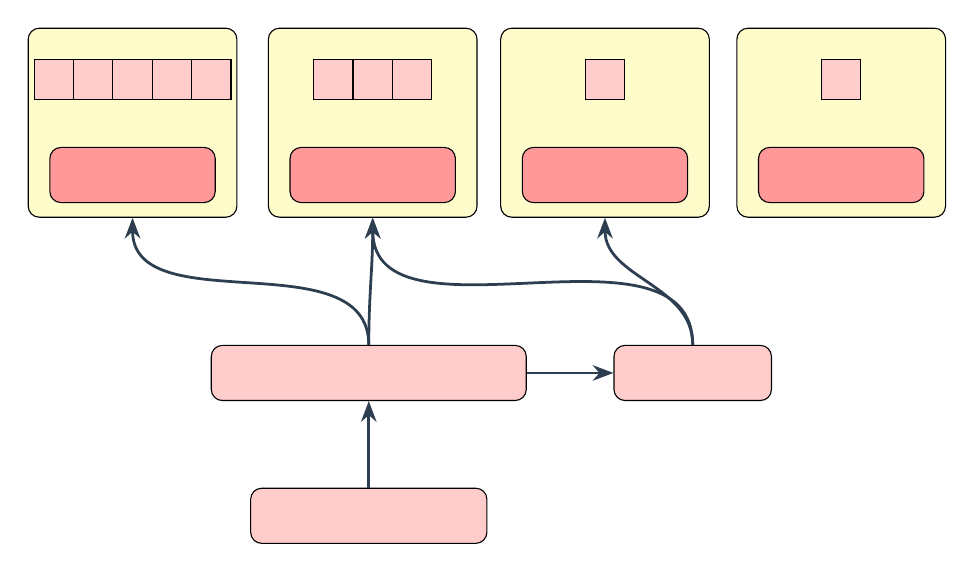
\begin{tikzpicture}[node distance=1.0mm and 1.0mm, >=Stealth, 
			wordnode/.style={draw=none, minimum height=5mm, inner sep=0pt},
			embnode/.style={draw=black, rounded corners, fill=red!20, minimum height=7mm, minimum width=30mm, inner sep=0pt},
			layernode/.style={draw=black, rounded corners, fill=red!20, minimum height=7mm, minimum width=20mm, inner sep=0pt},
			scoresnode/.style={draw=black, rounded corners, fill=red!40, minimum height=7mm, minimum width=21mm, inner sep=0pt},
			scorenode/.style={draw=black, fill=red!20, minimum height=5mm, minimum width=5mm, inner sep=0pt},
			chainLine/.style={line width=1pt,-, color=fontgray},
			scopebox/.style={draw=black, rounded corners, fill=yellow!20, minimum height = 24mm},
			scorebox/.style={draw=black,  rounded corners, fill=yellow!20, minimum height = 10mm, minimum width = 10mm},
			btag/.style={shape=circle, draw=black, rounded corners, fill=orange!20, minimum height=8mm, inner sep=0pt},
			atag/.style={shape=circle, draw=black, rounded corners, fill=orange!20, minimum height=8mm, inner sep=0pt},
			etag/.style={shape=circle, draw=black, rounded corners, fill=orange!20, minimum height=8mm, inner sep=0pt}
			]
			
			
\node [embnode] (emb)  [] {\color{black!80}\textsc{}};
			
			
			\node [wordnode, above=of emb, xshift=12mm, yshift=1mm] (bilstm)  [] {\color{black!80}\textsc{}};
			
			\node [layernode, above=of emb, minimum width=40mm, yshift=10mm, xshift=0mm] (lstm)  [] {\color{black!80}\textsc{}}; \node [layernode, right=of lstm, xshift=10mm] (segmental)  [] {\color{black!80}\textsc{}};
			
			
		
			\node [scoresnode, above=of lstm, yshift=17mm, xshift=-30mm] (f_t)  [] {\color{black!80}\textsc{}};
			\node [scoresnode, above=of lstm, yshift=17mm, xshift=0.5mm] (f_s)  [] {\color{black!80}\textsc{}};
			\node [scoresnode, above=of lstm, yshift=17mm, xshift=30mm] (f_g)  [] {\color{black!80}\textsc{}};
			\node [scoresnode, above=of lstm, yshift=17mm, xshift=60mm] (f_r)  [] {\color{black!80}\textsc{}};

			
			
			\node [scorenode, above=of f_s, yshift=5mm, fill=red!20, xshift=0mm] (f_s_plus)  [] {\color{black!80}\textsc{}};
			\node [scorenode, above=of f_s, yshift=5mm, fill=red!20, xshift=-5mm] (f_s_0)  [] {\color{black!80}\textsc{}};
			\node [scorenode, above=of f_s, yshift=5mm, fill=red!20, xshift=5mm] (f_s_minus)  [] {\color{black!80}\textsc{}};
			
			
			\node [scorenode, above=of f_t, yshift=5mm, fill=red!20, xshift=-10mm] (f_t_B)  [] {\color{black!80}\textsc{}};
			\node [scorenode, above=of f_t, yshift=5mm, fill=red!20, xshift=-5mm] (f_t_M)  [] {\color{black!80}\textsc{}};
			\node [scorenode, above=of f_t, yshift=5mm, fill=red!20, xshift=0mm] (f_t_E)  [] {\color{black!80}\textsc{}};
			\node [scorenode, above=of f_t, yshift=5mm, fill=red!20, xshift=5mm] (f_t_S)  [] {\color{black!80}\textsc{}};
			\node [scorenode, above=of f_t, yshift=5mm, fill=red!20, xshift=10mm] (f_t_O)  [] {\color{black!80}\textsc{}};
			
			
			\node [scorenode, above=of f_g, yshift=5mm, fill=red!20, xshift=0mm] (f_g_x)  [] {\color{black!80}\textsc{}};
			
			\node [scorenode, above=of f_r, yshift=5mm, fill=red!20, xshift=0mm] (f_r_x)  [] {\color{black!80}\textsc{}};
			
			


						

\begin{pgfonlayer}{background}
			\node [scopebox, above=of f_t, xshift=0mm, yshift=-10mm, text height=5mm, minimum width=26.5mm] (s_t)  [] {\color{blue!80}\textbf{\textsc{}}};
			\node [scopebox, above=of f_s, xshift=0mm, yshift=-10mm, text height=5mm, minimum width=26.5mm] (s_s)  [] {\color{blue!80}\textbf{\textsc{}}};
			\node [scopebox, above=of f_g, xshift=0mm, yshift=-10mm, text height=5mm, minimum width=26.5mm] (s_g)  [] {\color{blue!80}\textbf{\textsc{}}};
			\node [scopebox, above=of f_r, xshift=0mm, yshift=-10mm, text height=5mm, minimum width=26.5mm] (s_r)  [] {\color{blue!80}\textbf{\textsc{}}};
						
			\end{pgfonlayer}
			
			
			\draw[chainLine,->]   (emb) to[out=90,in=-90] (lstm);
			\draw[chainLine,->]   (lstm) to[out=0,in=180] (segmental);
			
			
			\draw[chainLine,->]   (lstm) to[out=90,in=-90] (s_t);
			\draw[chainLine,->]   (lstm) to[out=90,in=-90] (s_s);
			\draw[chainLine,->]   (segmental) to[out=90,in=-90] (s_s);
			\draw[chainLine,->]   (segmental) to[out=90,in=-90] (s_g);


			\end{tikzpicture} 
		}
\caption{Neural Module for Feature Score}
\label{fig:neural}
	\end{figure}
\subsubsection{Neural Module}

We deploy a simple LSTM-based neural architecture for learning features.
Given an input token sequence  of length , we first obtain the embedding sequence . As illustrated in Figure~\ref{fig:neural}, we then apply a bi-directional LSTM on the embedding sequence and obtain the hidden state  for each position , which could be represented as:
\setlength{\abovedisplayskip}{4pt} \setlength{\abovedisplayshortskip}{4pt}
\setlength{\belowdisplayskip}{4pt} \setlength{\belowdisplayshortskip}{4pt}

where  and  are the hidden states of the forward and backward LSTMs respectively.




Motivated by~\cite{wang2016graph, stern2017minimal}, we calculate the segment representation  for an opinion span with {\color{black}boundaries of  and  (both inclusive)} as follows:
\setlength{\abovedisplayskip}{4pt} \setlength{\abovedisplayshortskip}{4pt}
\setlength{\belowdisplayskip}{4pt} \setlength{\belowdisplayshortskip}{4pt}

where ,  and 



\subsubsection{Factorized Feature Score}
We explain how to compute the factorized feature scores (the second part of Equation~\ref{eq:score}) for the position-aware  tagging scheme based on the neural architecture described above.
Such factorized feature scores involve 4 types of scores, as illustrated in the solid boxes appearing in Figure~\ref{fig:neural} (top).


Basically, we calculate the factorized feature score for the tag  as follows:
\setlength{\abovedisplayskip}{4pt} \setlength{\abovedisplayshortskip}{4pt}
\setlength{\belowdisplayskip}{4pt} \setlength{\belowdisplayshortskip}{4pt}

where the linear layer  is used to calculate the score for local context for targets.
Such a linear layer takes the hidden state  as the input and returns a vector of length , with each value in the vector indicating the score of the corresponding sub-tag among . 
The subscript  indicates the index of such a sub-tag.

When , we need to calculate 3 additional factorized feature scores for capturing structural information by adding them to the basic score as follows:
\setlength{\abovedisplayskip}{3pt} \setlength{\abovedisplayshortskip}{3pt}
\setlength{\belowdisplayskip}{3pt} \setlength{\belowdisplayshortskip}{3pt}

Note that the subscript of the variable  is represented as  which are the absolute positions since  are the offsets. We explain such 3 additional factorized scores appearing in Equation~\ref{eq:triplet}. 




\begin{table*}[t]
\centering
\scalebox{0.64}{
\begin{tabular}{lrrrr|rrrr|rrrr|rrrr}
\toprule 
\multirow{2}{*}{\textbf{Dataset}} & \multicolumn{4}{c}{\texttt{14Rest}} & \multicolumn{4}{c}{\texttt{14Lap}} & \multicolumn{4}{c}{\texttt{15Rest}} & \multicolumn{4}{c}{\texttt{16Rest}} \\  
& \#S & \# + & \# 0 & \# - &  \#S & \# + & \# 0 & \# - & \#S & \# + & \# 0 & \# - & \#S & \# + & \# 0 & \# -  \\ \midrule
\textbf{Train} & 1266 & 1692 & 	166 & 	480 & 906  & 817 & 	126 & 	517 & 605 & 783 & 	25 & 	205  & 857 &  1015 & 	50 & 	329 \\ 
\textbf{Dev} & {\color{white}0,}310 & 404 & 	54 & 	119  & 219 &169 & 	36 & 	141 & 148 &185 & 	11 & 	53 & 210 &252 & 	11 & 	76 \\
\textbf{Test} & {\color{white}0,} 492 & 773 & 	66 & 	155 & 328 &364 & 	63 & 	116    & 322 &317 & 	25 & 	143& 326& 407 & 	29 & 	78  \\
\bottomrule
\end{tabular}
}
\vspace{-1mm}
\caption{Statistics of 4 datasets. (\#S denotes number of sentences, and \# +, \# 0, \# - denote numbers of positive, neutral and negative triplets respectively.)}
\label{tab:dataset}
\vspace{-1mm}
\end{table*}



\squishlist
\setlength\itemsep{0.5mm}


\item  calculates the score for the sentiment.
     A linear layer  takes the concatenation of the segment representation  for an opinion span and the local context  for a target, since we believe that the sentiment is mainly determined by the opinion span as well as the target phrase itself.
    Note that we only use the backward hidden state  here, because the end position of a target is not available in the tag and the target phrase appears on the right of this position .
    The linear layer  returns a vector of length , with each value representing the score of a certain polarity of . 
    The subscript  indicates the index of such a polarity.
    


\item  is used to calculate a score for an opinion span.
     A linear layer  takes the segment representation  of an opinion span and returns one number representing the score of an opinion span. 

\item  is used to calculate a score for offsets, since we believe the offset is an important feature.
     A linear layer  returns one number representing the score of offsets  which again are the distances between a target and two ends of the opinion span. 
    Here, we introduce the offset embedding  randomly initialized for encoding different offsets.
    Specifically, we calculate the score as follows\footnote{We use  since we care the offset between the starting positions of an opinion span and a target.}:
    \setlength{\abovedisplayskip}{4pt} \setlength{\abovedisplayshortskip}{4pt}
\setlength{\belowdisplayskip}{4pt} \setlength{\belowdisplayshortskip}{4pt}
    
    where  and  are learnable parameters.



\squishend







	




			


			




			
		


			
			


			


			




			


						





			


			








\subsection{One Target for Multiple Opinion Spans}
\label{sec:variant}


The approach \textbf{JET} described above allows multiple targets to point to the same opinion span.
One potential issue is that such an approach is not able to handle the case where one target is associated with multiple opinion spans. To remedy such an issue, we could swap a target and an opinion span to arrive at a new model as a model variant, since they are both text spans which are characterized by their boundaries.
Specifically, in such a model variant, we still use the extended tags  and , where we use sub-tags  to encode an opinion span, the offsets  for the target and  for the sentiment polarity.
We use a similar procedure for the feature score calculation.

\begin{figure}[t!]
		\centering
\adjustbox{max width=1.0\linewidth}{
			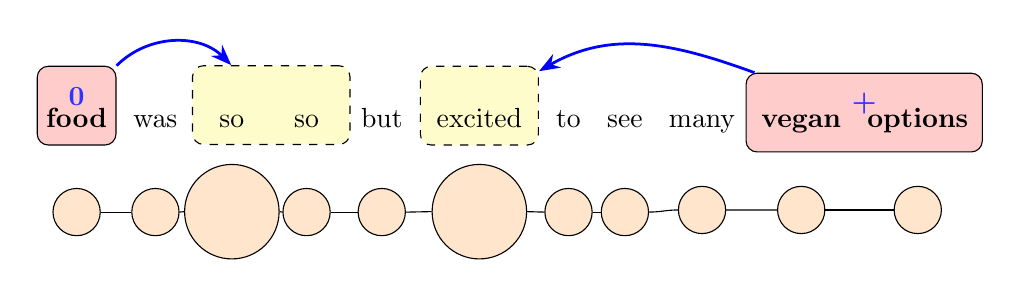
\begin{tikzpicture}[node distance=1.0mm and 1.0mm, >=Stealth, 
			wordnode/.style={draw=none, minimum height=5mm, inner sep=0pt},
			chainLine/.style={line width=1pt,->, color=blue},
			opinionbox/.style={draw=black, rounded corners, fill=yellow!20, dashed},
			targetbox/.style={draw=black, rounded corners, fill=red!20},
			BStag/.style={shape=circle, draw=black, rounded corners, fill=orange!20, minimum height=12mm, inner sep=0pt},
			MEOtag/.style={shape=circle, draw=black, rounded corners, fill=orange!20, minimum height=6mm, inner sep=0pt}
			]

\matrix (sent1) [matrix of nodes, nodes in empty cells, execute at empty cell=\node{\strut};]
			{
				\textbf{food} & [1mm] was &[3mm] so & [4mm]  so & [3mm] but &  [2mm]  excited & [2mm] to & [1mm] see & [1mm] many & [1mm] \textbf{vegan} & [1mm] \textbf{options}\\
};
			


\foreach \pos in {6}
				\node [BStag, below=of sent1-1-\pos, yshift=-2.4mm] (tag\pos)  [] {\color{black!80}\textsc{}};


\foreach \pos/\yoffset in {{2/-5.45},{5/-5.45},{1/-5.45},{7/-5.45},{8/-5.45},{9/-4.5},{10/-4.5},{11/-4.5}}
\node [MEOtag, below=of sent1-1-\pos, yshift=\yoffset mm] (tag\pos)  [] {\color{black!80}\textsc{}};
			
\node [BStag, below=of sent1-1-3, yshift=-2.4mm] (tag3)  [] {\color{black!80}\textsc{}};
			
\node [MEOtag, below=of sent1-1-4, yshift=-5.45mm] (tag4)  [] {\color{black!80}\textsc{}};

			\foreach \pos/\npos in {{1/2},{2/3},{3/4},{4/5},{5/6},{6/7},{7/8},{8/9},{9/10},{10/11}}
				\draw[-]  (tag\pos) to[out=0,in=180] (tag\npos);
							
			
						
			\begin{pgfonlayer}{background}
			
			\node [targetbox, above=of sent1-1-1, yshift=-7mm, text height=-2mm, minimum height = 10mm, minimum width=10mm] (e1)  [] {\color{blue!80}\textbf{\textsc{0}}};	
			\node [opinionbox, above=of sent1-1-3, xshift=5mm, yshift=-6mm, text height=-5mm, minimum height = 10mm, minimum width=20mm] (o1)  [] {\color{blue!80}\textbf{\textsc{}}};
			
			\draw[chainLine,->]   (e1) to[out=45,in=135] (o1);
			

			\node [targetbox, above=of sent1-1-10, xshift=8mm, yshift=-7mm, text height=-2mm, minimum height = 10mm, minimum width=30mm] (e2)  [] {\color{blue!80}\textbf{\textsc{+}}};			
			\node [opinionbox, above=of sent1-1-6, xshift=0mm, yshift=-7mm, text height=-5mm, minimum height = 10mm, minimum width=15mm] (o2)  [] {\color{blue!80}\textbf{\textsc{}}};		
			
			\draw[chainLine,->]  (e2) to[out=160,in=30] (o2);
				
			\end{pgfonlayer}
			
			
			
			\end{tikzpicture} 
		}		\caption{The gold tagging sequence of {\bf JET}\textsuperscript{o} for the example sentence.}
		\vspace{-1mm}
		\label{fig:tagging_o}
	\end{figure}





To differentiate with our first model, we name our first model as \textbf{JET} and such a model variant as \textbf{JET}.
The superscripts  and  indicate the use of the sub-tags  and  to encode a target and an opinion span respectively.
Figure~\ref{fig:tagging_o} presents the gold tagging sequence of \textbf{JET}.


































\subsection{Training and Inference}
The loss function  for the training data  is defined as:
\setlength{\abovedisplayskip}{-2pt} \setlength{\abovedisplayshortskip}{-2pt}
\setlength{\belowdisplayskip}{3pt} \setlength{\belowdisplayshortskip}{3pt}

The overall model is analogous to that of a neural CRF~\cite{NIPS2009_3869,do2010neural,lample2016neural}; hence the inference and decoding follow standard marginal and MAP inference\footnote{\textcolor{black}{See the Appendix for detailed algorithm.}} procedures.
For example, the prediction of  follows the Viterbi-like MAP inference procedure during decoding.
Notice that the number of labels at each position under the  position-aware tagging scheme is , since we need to compute segment representation for text spans of lengths within .
Hence, the time complexity for inference is .
{\color{black}When  (empirically, we found  can be up to 80 in our datasets, and we set ), this complexity is better than the existing work with complexity ~\cite{peng2019knowing}.}







\section{Experiments}




\subsection{Data}
\textcolor{black}{ 
We refine the dataset previously created by~\citet{peng2019knowing}\footnote{ \url{https://github.com/xuuuluuu/SemEval-Triplet-data}}.
We call our refined dataset  ASTE-Data-V2, and the original version as ASTE-Data-V1\footnote{We also report the results on ASTE-Data-V1 in the Appendix.}.
Note that ASTE-Data-V1 does not contain  cases where one opinion span is associated with multiple targets.
For example, there are two targets, ``\textit{service}'' and ``\textit{atmosphere}'', in the sentence ``\textit{Best service and atmosphere}''. The opinion span ``\textit{Best}'' is associated with such two targets, resulting in two triplets.
However, we found that not all such triplets are explicitly annotated in ASTE-Data-V1.
We refine the dataset with these additional missing triplets in our dataset ASTE-Data-V2\footnote{We also remove triplets with sentiment originally labeled as ``conflict'' by SemEval.}.
}








Table~\ref{tab:dataset} presents the detailed statistics for 4 datasets.\footnote{See the Appendix for more statistics.}
{\texttt{14Rest}}, {\texttt{15Rest}}, {\texttt{16Rest}} are the datasets of restaurant  domain and  {\texttt{14Lap}} is of laptop  domain.
Such datasets were all created based on the datasets originally released by SemEval~\cite{pontiki-EtAl:2014:SemEval,pontiki-etal-2015-semeval,pontiki2016semeval, fan-etal-2019-target}.

























\begin{table*}[!t]


    \centering
\scalebox{0.62}{
    \begin{tabular}{lcccc|cccc|cccc|cccc}
\toprule
      \multirow{2}{*}{\textbf{Models}} & \multicolumn{4}{c}{\texttt{14Rest}} & \multicolumn{4}{c}{\texttt{14Lap}} & \multicolumn{4}{c}{\texttt{15Rest}}  & \multicolumn{4}{c}{\texttt{16Rest}}    \\ &Dev  &  &  & &Dev  &  &  & &Dev  &  &  &  &Dev  &  &  &  \\ \midrule
       
        \textbf{CMLA+} & -& 39.18 & 47.13 & 42.79 &-&  30.09 & 36.92 & 33.16 &-&  34.56 & 39.84 & 37.01 &-&  41.34 & 42.10 & 41.72          \\
        \textbf{RINANTE+} &-&  31.42 & 39.38 & 34.95 &-&  21.71 & 18.66 & 20.07  &-&  29.88 & 30.06 & 29.97 &-&  25.68 & 22.30 & 23.87  \\
        \textbf{Li-unified-R} &-&  41.04 & 67.35 & 51.00 &-&  40.56 & 44.28 & 42.34 &-&  44.72 & 51.39 & 47.82 &-&  37.33 & 54.51 & 44.31 \\
        \citet{peng2019knowing} &-&  43.24 & 63.66 & 51.46 &-&  37.38 & 50.38 & 42.87 &-&  48.07 & 57.51 & 52.32 &-&  46.96 & 64.24 & 54.21 \\ 
\midrule
        \textbf{JET} & 
        45.67 & 72.46 & 32.29 & 44.68 & 35.69 & 57.39 & 24.31 & 34.15 & 42.34 &  64.81 & 28.87 & 39.94 & 43.27 & 68.75 & 38.52 & 49.38 \\
        \textbf{JET} &
        50.87 & 70.02 & 42.76 & 53.09 & 42.34 &  56.86 & 31.31 & 40.38 & 52.02 & 59.87 & 36.91 & 45.66 & 52.13 & 67.22 & 47.47 & 55.64 \\
        \textbf{JET}  &
        50.31 & 69.67 & 47.38 & 56.41 & 45.90 & 48.77 & 32.78 & 39.21 & 52.50 & 64.50 & 40.82 & 50.00 & 57.69 & 64.64 & 47.67 & 54.87 \\
        
        \textbf{JET} &52.41 & 62.23 & 48.39 & 54.44 & \underline{48.26} &  54.84 & 34.44 & \bf{42.31} & 54.97 & 55.67 & 43.51 & 48.84 & 57.83 & 61.63 & 48.44 & 54.25 \\
        \textbf{JET} &\underline{53.14}& 66.76&49.09& \bf{56.58}& 47.68& 52.00& 35.91 &42.48 &\underline{55.06}& 59.77&42.27& \bf{49.52}& \underline{58.45} &63.59&50.97&\bf{56.59}\1.5mm]
\textbf{JET} &45.02&  66.30 & 35.38& 46.14 &33.01&  50.43 & 23.88 & 32.41 &46.80&  58.88 & 25.49 & 35.58&40.33& 60.47 & 39.14 & 47.52 \\        
        \textbf{JET} &53.14&  62.31 & 43.16& 50.99 &38.99& 55.37 & 33.67 & 41.88&54.59&  55.99 & 38.02 & 45.29 &47.87& 69.45 & 46.45 & 55.67\\
        \textbf{JET} &58.19& 63.84 & 52.44 & 57.58 &40.87& 49.86& 36.33& 42.03 &57.14&  57.57 & 42.64& 48.99&53.99& 73.98 &54.41 & 62.70\\  
        \textbf{JET} &57.94&  64.31 &	54.99 &	59.29 &\underline{43.23}& 52.36& 40.82& \bf{45.87} &59.51&  52.02 & 48.13 & {50.00} &\underline{56.08}& 66.91 & 58.71 & \bf{62.54}\\
        \textbf{JET} &\underline{58.66}& 62.26&	56.84&\bf{59.43}& 42.50&52.01	&39.59&	44.96 &\underline{60.32}&63.25&	46.15&	\bf{53.37}&55.63& 66.58 & 57.85 & 61.91\\ [1.5mm] \multicolumn{4}{l}{\textbf{+ Contextualized Word Representation (BERT)}}& & &&&&&&&&&&&\\
        \textbf{JET} & 61.01&  70.20	& 53.02& 60.41 & 49.07 & 51.48 & 42.65 & 46.65 & 62.96 & 62.14 & 47.25	& 53.68 & 60.41 & 71.12	& 57.20	& 63.41 \\
        \textbf{JET}  & 60.86 & 67.97	& 60.32	& 63.92 & 45.76 & 58.47	& 43.67	& 50.00  & 64.12 & 58.35 & 51.43 & 54.67 & 60.17 & 64.77 & 61.29 & 62.98 \\
        
\bottomrule
    \end{tabular}
    }
\caption{The experimental results on the previous released datasets ASTE-Data-V1. The underlined scores indicate the best results on the dev set, and the highlighted scores are the corresponding test  results. }
    \label{tab:main_results_1}
    \vspace{-4mm}
\end{table*}

\section{Decoding based on Viterbi}
Let  as the new tag set under our position-aware tagging scheme, where  denotes the sentiment polarity for the target, and   indicate the position information which are the distances between the two ends of an opinion span and the starting position of a target respectively.

As we know, , .

 

We define the sub-tags of  as  and  respectively, and the sub-tags of  as themselves.
We use the bar on top to denote the sub-tag.
For example,  is the subtag of .





We use  to denote the score for the optimal sequence  among all the possible sequences whose last tag is .

Given the input  of length , we aim to obtain the optimal sequence . \\
\begin{itemize}
    \item Base Case for all the  \\
If :
    
    
    If :
    \setlength{\abovedisplayskip}{4pt} \setlength{\abovedisplayshortskip}{4pt}
    \setlength{\belowdisplayskip}{4pt} \setlength{\belowdisplayshortskip}{4pt}
    
where  , , , and  are the factorized feature score  mentioned in the section 2.2.2.
    \item Loop forward for  and all the  \\
    If :
    \setlength{\abovedisplayskip}{4pt} \setlength{\abovedisplayshortskip}{4pt}
    \setlength{\belowdisplayskip}{4pt} \setlength{\belowdisplayshortskip}{4pt}
    
    If :
    \setlength{\abovedisplayskip}{4pt} \setlength{\abovedisplayshortskip}{4pt}
    \setlength{\belowdisplayskip}{4pt} \setlength{\belowdisplayshortskip}{4pt}
    
    \item Backtrack for the optimal sequence  \\
    \setlength{\abovedisplayskip}{4pt} \setlength{\abovedisplayshortskip}{4pt}
    \setlength{\belowdisplayskip}{4pt} \setlength{\belowdisplayshortskip}{4pt}
    
    Loop for  
    
\end{itemize}
Note that  appears before the start of the input sentence and  appears after the end of the input sentence.

The time complexity is .


\section{Analysis}
\subsection{Robustness Analysis}
We present the performance on targets, opinion spans and offsets of different lengths for two models \textbf{JET} and \textbf{JET} with BERT on 3 datasets {\texttt{14Lap}},{\texttt{15Rest}} and {\texttt{16Rest}} in Figure~\ref{fig:f1_diff_lengths_14lap}, Figure~\ref{fig:f1_diff_lengths_15rest} and Figure~\ref{fig:f1_diff_lengths_16rest} respectively.
\subsection{Qualitative Analysis}

We present one additional example sentence selected from the test data as well as predictions by~\citet{peng2019knowing}, \textbf{JET} and \textbf{JET} in Table~\ref{tab:qualitative2}.
As we can see, the gold data contains two triplets.
\citet{peng2019knowing} only predicts 1 opinion span, and therefore incorrectly assigns the opinion span ``Good'' to the target ``price''.
\textbf{JET} is able to make the correct predictions.
\textbf{JET} only predicts 1 triplet correctly.
The qualitative analysis helps us to better understand the differences among these models.

\section{More Related Work}
The task of joint entity and relation extraction is also related to joint triplet extraction.
Different from our task, such a relation extraction task aims to extract a pair of entities (instead of a target and an opinion span) and their relation as a triplet in a joint manner.
\citet{miwa-sasaki-2014-modeling} and \citet{li-ji-2014-incremental} used approaches motivated by a table-filling method to jointly extract entity pairs as well as their relations.
The tree-structured neural networks~\cite{miwa-bansal-2016-end} and CRF-based approaches~\cite{adel-schutze-2017-global} were also adopted to capture rich context information for triplet extraction.
Recently, \citet{bekoulis-etal-2018-adversarial} used adversarial training~\cite{goodfellow15} for this task and results show that it performs more robustly in different domains.
Although these approaches may not be applied to our task ASTE, they may provide inspirations for future work. 


\begin{table*}[t!]
     \centering
     \scalebox{0.8}{
     \begin{tabular}{ c  c c c   }
     \toprule
      Gold & \citet{peng2019knowing} & \textbf{JET} & \textbf{JET} \\ 
\midrule
            \scalebox{0.7}{
     	    	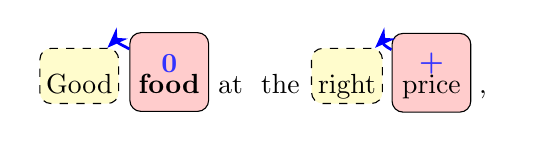
\begin{tikzpicture}[node distance=1.0mm and 1.0mm, >=Stealth, 
			wordnode/.style={draw=none, minimum height=2mm, inner sep=0pt},
			chainLine/.style={line width=1pt,->, color=blue},
			opinionbox/.style={draw=black, rounded corners, fill=yellow!20, dashed},
			targetbox/.style={draw=black, rounded corners, fill=red!20},
			]

\matrix (sent1) [matrix of nodes, ampersand replacement=\&, nodes in empty cells, execute at empty cell=\node{\strut};]
			{
				Good \& [1mm] \textbf{food} \&  at \&  the \&  right \&  [1mm] price \& ,  \\
			};
			
			
			\begin{pgfonlayer}{background}
			
			\node [targetbox, above=of sent1-1-2, yshift=-7mm, text height=-2mm, minimum height = 10mm, minimum width=10mm] (e1)  [] {\color{blue!80}\textbf{\textsc{0}}};	
			\node [opinionbox, above=of sent1-1-1, xshift=0mm, yshift=-6mm, text height=-5mm, minimum height = 7mm, minimum width=10mm] (o1)  [] {\color{blue!80}\textbf{\textsc{}}};
			
			\draw[chainLine,->]   (e1) to[out=150,in=45] (o1);
			

			\node [targetbox, above=of sent1-1-6, xshift=0mm, yshift=-7mm, text height=-2mm, minimum height = 10mm, minimum width=10mm] (e2)  [] {\color{blue!80}\textbf{\textsc{+}}};			
			\node [opinionbox, above=of sent1-1-5, xshift=0mm, yshift=-6mm, text height=-5mm, minimum height = 7mm, minimum width=9mm] (o2)  [] {\color{blue!80}\textbf{\textsc{}}};		
			
			\draw[chainLine,->]  (e2) to[out=150,in=45] (o2);
				
			\end{pgfonlayer}
			
			\end{tikzpicture} 
			}
			
     
      & 
      
       \scalebox{0.7}{
     	    	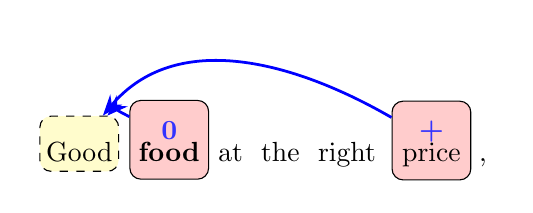
\begin{tikzpicture}[node distance=1.0mm and 1.0mm, >=Stealth, 
			wordnode/.style={draw=none, minimum height=2mm, inner sep=0pt},
			chainLine/.style={line width=1pt,->, color=blue},
			opinionbox/.style={draw=black, rounded corners, fill=yellow!20, dashed},
			targetbox/.style={draw=black, rounded corners, fill=red!20},
			]

\matrix (sent1) [matrix of nodes, ampersand replacement=\&, nodes in empty cells, execute at empty cell=\node{\strut};]
			{
				Good \&  [1mm] \textbf{food} \&  at \&  the \&  right \&  [1mm] price \& ,  \\
			};
			
			
			\begin{pgfonlayer}{background}
			
			\node [targetbox, above=of sent1-1-2, yshift=-7mm, text height=-2mm, minimum height = 10mm, minimum width=10mm] (e1)  [] {\color{blue!80}\textbf{\textsc{0}}};	
			\node [opinionbox, above=of sent1-1-1, xshift=0mm, yshift=-6mm, text height=-5mm, minimum height = 7mm, minimum width=10mm] (o1)  [] {\color{blue!80}\textbf{\textsc{}}};
			
			\draw[chainLine,->]   (e1) to[out=150,in=45] (o1);
			

			\node [targetbox, above=of sent1-1-6, xshift=0mm, yshift=-7mm, text height=-2mm, minimum height = 10mm, minimum width=10mm] (e2)  [] {\color{blue!80}\textbf{\textsc{+}}};			


			\draw[chainLine,->]  (e2) to[out=150,in=50] (o1);
				
			\end{pgfonlayer}
			
			\end{tikzpicture} 
			}
     
      & 
      
       \scalebox{0.7}{
     	    	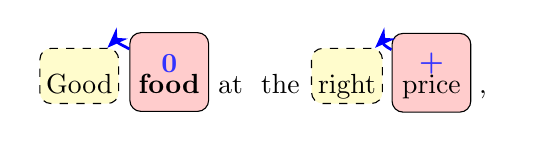
\begin{tikzpicture}[node distance=1.0mm and 1.0mm, >=Stealth, 
			wordnode/.style={draw=none, minimum height=2mm, inner sep=0pt},
			chainLine/.style={line width=1pt,->, color=blue},
			opinionbox/.style={draw=black, rounded corners, fill=yellow!20, dashed},
			targetbox/.style={draw=black, rounded corners, fill=red!20},
			]

\matrix (sent1) [matrix of nodes, ampersand replacement=\&, nodes in empty cells, execute at empty cell=\node{\strut};]
			{
				Good \&  [1mm] \textbf{food} \&  at \&  the \&  right \&  [1mm]  price \& ,  \\
			};
			
			
			\begin{pgfonlayer}{background}
			
			\node [targetbox, above=of sent1-1-2, yshift=-7mm, text height=-2mm, minimum height = 10mm, minimum width=10mm] (e1)  [] {\color{blue!80}\textbf{\textsc{0}}};	
			\node [opinionbox, above=of sent1-1-1, xshift=0mm, yshift=-6mm, text height=-5mm, minimum height = 7mm, minimum width=10mm] (o1)  [] {\color{blue!80}\textbf{\textsc{}}};
			
			\draw[chainLine,->]   (e1) to[out=150,in=45] (o1);
			

			\node [targetbox, above=of sent1-1-6, xshift=0mm, yshift=-7mm, text height=-2mm, minimum height = 10mm, minimum width=10mm] (e2)  [] {\color{blue!80}\textbf{\textsc{+}}};			
			\node [opinionbox, above=of sent1-1-5, xshift=0mm, yshift=-6mm, text height=-5mm, minimum height = 7mm, minimum width=9mm] (o2)  [] {\color{blue!80}\textbf{\textsc{}}};		
			
			\draw[chainLine,->]  (e2) to[out=150,in=45] (o2);
				
			\end{pgfonlayer}
			
			\end{tikzpicture} 
			}
    
     &

 \scalebox{0.7}{
     	    	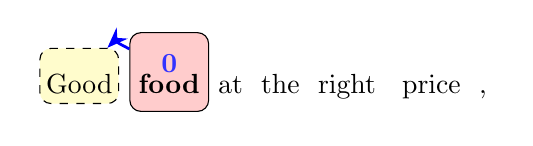
\begin{tikzpicture}[node distance=1.0mm and 1.0mm, >=Stealth, 
			wordnode/.style={draw=none, minimum height=2mm, inner sep=0pt},
			chainLine/.style={line width=1pt,->, color=blue},
			opinionbox/.style={draw=black, rounded corners, fill=yellow!20, dashed},
			targetbox/.style={draw=black, rounded corners, fill=red!20},
			]

\matrix (sent1) [matrix of nodes, ampersand replacement=\&, nodes in empty cells, execute at empty cell=\node{\strut};]
			{
				Good \&  [1mm] \textbf{food} \&  at \&  the \&  right \&  [1mm] price \& ,  \\
			};
			
			
			\begin{pgfonlayer}{background}
			
			\node [targetbox, above=of sent1-1-2, yshift=-7mm, text height=-2mm, minimum height = 10mm, minimum width=10mm] (e1)  [] {\color{blue!80}\textbf{\textsc{0}}};	
			\node [opinionbox, above=of sent1-1-1, xshift=0mm, yshift=-6mm, text height=-5mm, minimum height = 7mm, minimum width=10mm] (o1)  [] {\color{blue!80}\textbf{\textsc{}}};
			
			\draw[chainLine,->]   (e1) to[out=150,in=45] (o1);
			





			\end{pgfonlayer}
			
			\end{tikzpicture} 
			}
      \\ 
      
			




			

















			

















			

















			













\bottomrule
      \end{tabular}
      }
      \centering
\caption{Qualitative Analysis}
      \label{tab:qualitative2}
\end{table*}

\begin{algorithm}[H]
\SetAlgoLined
Initialization\;
\For{}{
\For{ }
{ \; \\
}
\For{ }{
    \For{}{
        \For{}{
            \For{}{
            \;\\
            {}}}}}
}
Loop Forward\;
\For{}{
\For{ }
{\; \\
 \\
}

\For{ }{
    \For{}{
        \For{}{
            \For{}{
            \;\\
            {}}}}}
}


Backward for the optimal sequence \;
\For{} {
\If{}{}
\Else{}
}
\caption{Decoding based on Viterbi}
\end{algorithm}







\begin{figure}[t!]
\centering
\begin{subfigure}{0.45\linewidth}
   \centering
    \begin{adjustwidth}{-0.4cm}{0.0cm}
    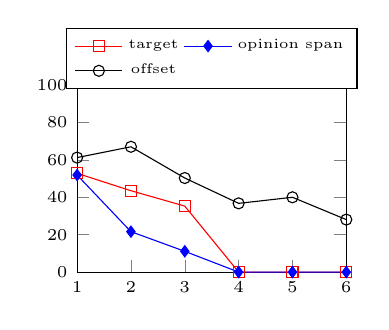
\begin{tikzpicture}
    \pgfplotsset{width=5cm,compat=1.9}
    \begin{axis}
[
                title={},
legend style={font=\fontsize{5}{1}\selectfont},
                legend style={at={(0.5,0.85)},anchor=south,legend columns=2}, 
                xticklabel style = {font=\fontsize{6}{1}\selectfont},
                yticklabel style = {font=\fontsize{6}{1}\selectfont},
xmin=1, xmax=6,
                ymin=0, ymax=115,
                xtick={1,2,3,4,5,6,7},
                xticklabels = {1,2,3,4,5,6,},
                ytick={0.0,20,40,60, 80,100},
]
    \addplot [mark=square, color=red] plot coordinates {
        (1,52.82) (2, 43.51) (3, 35.29) (4, 0) (5, 0)(6, 0)};
        \addplot [mark=diamond*, color=blue] plot coordinates {
        (1, 51.90) (2, 21.62) (3,11.11)  (4,0) (5,0) (6, 0) };
        \addplot[mark=o, color=black] plot coordinates {
        (1, 61.24) (2, 67.01) (3, 50.31) ( 4, 36.76) (5, 40) (6, 28.07)};
    \legend{target \\opinion span\\ offset\\}
    \end{axis}
    \end{tikzpicture}
    \vspace{-5mm}
    \end{adjustwidth}
    \centering
    \vspace{-2mm}
    \caption{\textbf{JET}}
\end{subfigure}
\hfill
\begin{subfigure}{0.45\linewidth}
   \centering
   \begin{adjustwidth}{-0.6cm}{0.0cm}
        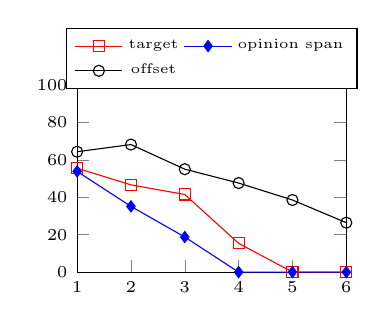
\begin{tikzpicture}
        \pgfplotsset{width=5cm,compat=1.9}
        \begin{axis}
[
                    title={},
legend style={font=\fontsize{5}{1}\selectfont}, legend style={at={(0.5,0.85)},anchor=south,legend columns=2}, 
                    xticklabel style = {font=\fontsize{6}{1}\selectfont},
                    yticklabel style = {font=\fontsize{6}{1}\selectfont},
xmin=1, xmax=6,
                    ymin=0, ymax=115,
                    xtick={1,2,3,4,5,6},
                    xticklabels = {1,2,3,4,5,6},
                    ytick={0.0,20,40,60, 80,100},
]
        \addplot [mark=square, color=red] plot coordinates {
        (1,55.57) (2, 46.65) (3, 41.51) (4, 15.38) (5, 0)(6, 0)(7, 0)};
        \addplot [mark=diamond*, color=blue] plot coordinates {
        (1, 53.85) (2, 35.14) (3, 18.75)  (4, 0) (5,0) (6, 0)(7, 0) };
        \addplot[mark=o, color=black] plot coordinates {
        (1, 64.37) (2, 68.20) (3, 55.03) ( 4, 47.62) (5, 38.55) (6, 26.42)};
        \legend{target \\opinion span\\ offset\\}
        \end{axis}
        \end{tikzpicture}
        \vspace{-5mm}
    \end{adjustwidth}
    \centering
    \vspace{-2mm}
   \caption{\textbf{JET}}
   
\end{subfigure}
\centering
\caption{ scores (-axis) of different lengths (-axis) for targets, opinion spans and offsets on the dataset {\texttt{14Lap}}.}
\label{fig:f1_diff_lengths_14lap}
\end{figure}





\begin{figure}[t!]
\centering
\begin{subfigure}{0.45\linewidth}
   \centering
    \begin{adjustwidth}{-0.4cm}{0.0cm}
    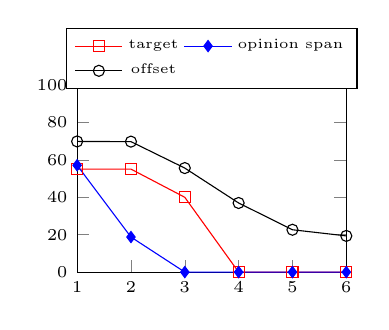
\begin{tikzpicture}
    \pgfplotsset{width=5cm,compat=1.9}
    \begin{axis}
[
                title={},
legend style={font=\fontsize{5}{1}\selectfont},
                legend style={at={(0.5,0.85)},anchor=south,legend columns=2}, 
                xticklabel style = {font=\fontsize{6}{1}\selectfont},
                yticklabel style = {font=\fontsize{6}{1}\selectfont},
xmin=1, xmax=6,
                ymin=0, ymax=115,
                xtick={1,2,3,4,5,6,7},
                xticklabels = {1,2,3,4,5,6,},
                ytick={0.0,20,40,60, 80,100},
]
        \addplot [mark=square, color=red] plot coordinates {
        (1,55.08) (2, 55.08) (3, 40) (4, 0) (5, 0)(6, 0)};
        \addplot [mark=diamond*, color=blue] plot coordinates {
        (1, 57.14) (2, 18.75) (3,0)  (4,0) (5,0) (6, 0) };
        \addplot[mark=o, color=black] plot coordinates {
        (1, 69.87) (2, 69.77) (3, 55.63) ( 4, 36.96) (5, 22.64) (6, 19.35)};
    \legend{target \\opinion span\\ offset\\}
    \end{axis}
    \end{tikzpicture}
    \vspace{-5mm}
    \end{adjustwidth}
    \centering
    \vspace{-2mm}
    \caption{\textbf{JET}}
\end{subfigure}
\hfill
\begin{subfigure}{0.45\linewidth}
   \centering
   \begin{adjustwidth}{-0.6cm}{0.0cm}
        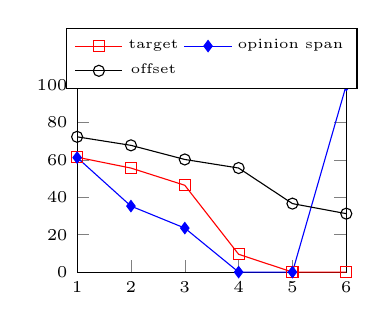
\begin{tikzpicture}
        \pgfplotsset{width=5cm,compat=1.9}
        \begin{axis}
[
                    title={},
legend style={font=\fontsize{5}{1}\selectfont}, legend style={at={(0.5,0.85)},anchor=south,legend columns=2}, 
                    xticklabel style = {font=\fontsize{6}{1}\selectfont},
                    yticklabel style = {font=\fontsize{6}{1}\selectfont},
xmin=1, xmax=6,
                    ymin=0, ymax=115,
                    xtick={1,2,3,4,5,6},
                    xticklabels = {1,2,3,4,5,6},
                    ytick={0.0,20,40,60, 80,100},
]
        \addplot [mark=square, color=red] plot coordinates {
        (1, 61.44) (2, 55.63) (3, 46.43) (4, 9.52) (5, 0)(6, 0)};
        \addplot [mark=diamond*, color=blue] plot coordinates {
        (1, 61.25) (2, 35.29) (3, 23.53)  (4,0) (5, 0) (6, 100) };
        \addplot[mark=o, color=black] plot coordinates {
        (1, 72.34) (2, 67.78) (3, 60.23) ( 4, 55.65) (5, 36.62) (6, 31.25)};
        \legend{target \\opinion span\\ offset\\}
        \end{axis}
        \end{tikzpicture}
        \vspace{-5mm}
    \end{adjustwidth}
    \centering
    \vspace{-2mm}
   \caption{\textbf{JET}}
\end{subfigure}
\centering
\caption{ scores (-axis) of different lengths (-axis) for targets, opinion spans and offsets on the dataset {\texttt{15Rest}}.}
\label{fig:f1_diff_lengths_15rest}
\end{figure}



\begin{figure}[t!]
\centering
\begin{subfigure}{0.45\linewidth}
   \centering
    \begin{adjustwidth}{-0.4cm}{0.0cm}
    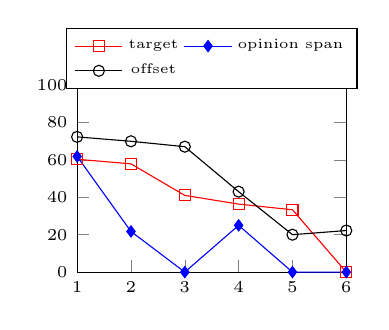
\begin{tikzpicture}
    \pgfplotsset{width=5cm,compat=1.9}
    \begin{axis}
[
                title={},
legend style={font=\fontsize{5}{1}\selectfont},
                legend style={at={(0.5,0.85)},anchor=south,legend columns=2}, 
                xticklabel style = {font=\fontsize{6}{1}\selectfont},
                yticklabel style = {font=\fontsize{6}{1}\selectfont},
xmin=1, xmax=6,
                ymin=0, ymax=115,
                xtick={1,2,3,4,5,6,7},
                xticklabels = {1,2,3,4,5,6,},
                ytick={0.0,20,40,60, 80,100},
]
    \addplot [mark=square, color=red] plot coordinates {
    (1,60.34) (2, 57.89) (3, 41.02) (4, 36.36) (5, 33.33)(6, 0)(7, 0)};
    \addplot [mark=diamond*, color=blue] plot coordinates {
    (1, 61.87) (2, 21.74) (3, 0)  (4, 25) (5,0) (6, 0)(7, 0) };
    \addplot [mark=o, color=black] plot coordinates {
    (1, 72.31) (2, 69.95) (3, 67.07) ( 4, 43.01) (5, 20.00) (6, 22.22)(7, 0) };
    \legend{target \\opinion span\\ offset\\}
    \end{axis}
    \end{tikzpicture}
    \end{adjustwidth}
    \centering
    \vspace{-3mm}
    \caption{\textbf{JET}}
    \vspace{-2mm}
\end{subfigure}
\hfill
\begin{subfigure}{0.45\linewidth}
   \centering
   \begin{adjustwidth}{-0.6cm}{0.0cm}
        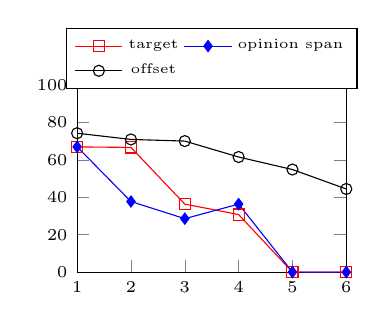
\begin{tikzpicture}
        \pgfplotsset{width=5cm,compat=1.9}
        \begin{axis}
[
                    title={},
legend style={font=\fontsize{5}{1}\selectfont}, legend style={at={(0.5,0.85)},anchor=south,legend columns=2}, 
                    xticklabel style = {font=\fontsize{6}{1}\selectfont},
                    yticklabel style = {font=\fontsize{6}{1}\selectfont},
xmin=1, xmax=6,
                    ymin=0, ymax=115,
                    xtick={1,2,3,4,5,6},
                    xticklabels = {1,2,3,4,5,6},
                    ytick={0.0,20,40,60, 80,100},
]
        \addplot [mark=square, color=red] plot coordinates {
        (1,66.95) (2, 66.67) (3, 36.36) (4, 30.77) (5, 0)(6, 0)};
        \addplot [mark=diamond*, color=blue] plot coordinates {
        (1, 66.98) (2, 37.74) (3, 28.57)  (4, 36.36) (5,0) (6, 0) };
        \addplot[mark=o, color=black] plot coordinates {
        (1, 74.27) (2, 70.94) (3, 70.06) ( 4, 61.54) (5, 54.84) (6, 44.44)};
        \legend{target \\opinion span\\ offset\\}
        \end{axis}
        \end{tikzpicture}
        
    \end{adjustwidth}
    \centering
    \vspace{-3mm}
   \caption{\textbf{JET}}
  \vspace{-2mm}
\end{subfigure}
\centering
\caption{ scores (-axis) of different lengths (-axis) for targets, opinion spans and offsets on the dataset {\texttt{16Rest}}.}
\label{fig:f1_diff_lengths_16rest}
\vspace{-2mm}
\end{figure}




































	

















\end{document}